\begin{tikzpicture}
	\pgfplotsset{/tikz/font={\small}}
	\begin{axis}[
		grid=both,
		width=1.0\textwidth,
		height=0.3\textheight,
		x tick label style={
		/pgf/number format/1000 sep=},
		ytick={0,...,-13},
		y tick label style={
			/pgf/number format/.cd,
			fixed,
			fixed zerofill,
			precision=1,
		},
		y dir=reverse,
		ymax=0.5, ymin=-13,
		ylabel={Y BD-rate (\%)},
		% enlargelimits=0.15,
		enlarge y limits=false,
		enlarge x limits=0.04,
		legend style={at={(0.5,-0.45)},
		anchor=north,legend columns=-1},
		ybar,
		bar width=1pt,
		xtick=data,
		xtick align=inside,
		% nodes near coords,
		% xlabel={Sequences},
		% xlabel near ticks,
		symbolic x coords={
			NebutaFestival,
			PeopleOnStreet,
			SteamLocTrain,
			Traffic,
			BasketballDrive,
			BQTerrace,
			Cactus,
			Kimono1,
			ParkScene,
			BasketballDrill,
			BQMall,
			PartyScene,
			RaceHorses\_480p,
			BasketballPass,
			BlowingBubbles,
			BQSquare,
			RaceHorses\_240p,
			FourPeople,
			Johnny,
			KristenAndSara,
			BasketDrillText,
			ChinaSpeed,
			SlideEditing,
			SlideShow,
			Overall,
		},
		x tick label style={rotate=-60,anchor=west},
		]

		\addlegendentry{Sep AI}
		\addplot coordinates {
		(NebutaFestival,   -0.34)
		(PeopleOnStreet,   -1.40)
		(SteamLocTrain,    -0.36)
		(Traffic,          -1.68)
		(BasketballDrive,  -1.17)
		(BQTerrace,        -1.80)
		(Cactus,           -1.95)
		(Kimono1,          -0.46)
		(ParkScene,        -1.68)
		(BasketballDrill,  -2.09)
		(BQMall,           -2.04)
		(PartyScene,       -2.18)
		(RaceHorses\_480p, -1.71)
		(BasketballPass,   -1.68)
		(BlowingBubbles,   -1.96)
		(BQSquare,         -2.26)
		(RaceHorses\_240p, -1.57)
		(FourPeople,       -1.83)
		(Johnny,           -1.29)
		(KristenAndSara,   -1.34)
		(BasketDrillText,  -2.37)
		(ChinaSpeed,       -2.02)
		(SlideEditing,     -2.04)
		(SlideShow,        -2.53)
		(Overall,          -1.66)
		};

		\addlegendentry{Sep RA}
		\addplot coordinates {
		(NebutaFestival,   -0.05)
		(PeopleOnStreet,   -0.48)
		(SteamLocTrain,     0.33)
		(Traffic,          -1.25)
		(BasketballDrive,  -0.35)
		(BQTerrace,        -1.08)
		(Cactus,           -1.15)
		(Kimono1,          -0.25)
		(ParkScene,        -1.09)
		(BasketballDrill,  -1.32)
		(BQMall,           -1.20)
		(PartyScene,       -1.40)
		(RaceHorses\_480p, -0.70)
		(BasketballPass,   -0.82)
		(BlowingBubbles,   -1.21)
		(BQSquare,         -1.21)
		(RaceHorses\_240p, -0.58)
		(FourPeople,       -1.94)
		(Johnny,           -1.61)
		(KristenAndSara,   -1.75)
		(BasketDrillText,  -1.51)
		(ChinaSpeed,       -1.22)
		(SlideEditing,     -2.18)
		(SlideShow,        -2.32)
		(Overall,          -1.10)
		};

		\addlegendentry{N-sep AI}
		\addplot coordinates {
		(NebutaFestival,   -0.52)
		(PeopleOnStreet,   -2.76)
		(SteamLocTrain,    -0.46)
		(Traffic,          -3.07)
		(BasketballDrive,  -3.15)
		(BQTerrace,        -5.11)
		(Cactus,           -3.75)
		(Kimono1,          -1.06)
		(ParkScene,        -2.20)
		(BasketballDrill, -12.83)
		(BQMall,           -3.27)
		(PartyScene,       -3.31)
		(RaceHorses\_480p, -3.99)
		(BasketballPass,   -3.71)
		(BlowingBubbles,   -4.21)
		(BQSquare,         -3.72)
		(RaceHorses\_240p, -4.61)
		(FourPeople,       -3.42)
		(Johnny,           -2.96)
		(KristenAndSara,   -3.49)
		(BasketDrillText, -11.01)
		(ChinaSpeed,       -2.87)
		(SlideEditing,     -1.82)
		(SlideShow,        -3.49)
		(Overall,          -3.78)
		};

		\addlegendentry{N-sep RA}
		\addplot coordinates {
		(NebutaFestival,  -0.04)
		(PeopleOnStreet,  -1.16)
		(SteamLocTrain,   -0.10)
		(Traffic,         -2.32)
		(BasketballDrive, -1.76)
		(BQTerrace,       -2.83)
		(Cactus,          -2.42)
		(Kimono1,         -0.50)
		(ParkScene,       -1.50)
		(BasketballDrill, -7.06)
		(BQMall,          -1.91)
		(PartyScene,      -2.29)
		(RaceHorses\_480p,-2.16)
		(BasketballPass,  -1.97)
		(BlowingBubbles,  -2.35)
		(BQSquare,        -2.00)
		(RaceHorses\_240p,-2.03)
		(FourPeople,      -3.27)
		(Johnny,          -2.86)
		(KristenAndSara,  -3.26)
		(BasketDrillText, -6.31)
		(ChinaSpeed,      -1.58)
		(SlideEditing,    -1.97)
		(SlideShow,       -2.96)
		(Overall,         -2.36)
		};

	\end{axis}
\end{tikzpicture}
